\documentclass[14pt,a4paper]{extarticle}

\usepackage[T1]{fontenc}
\usepackage[utf8]{inputenc}
\usepackage[polish]{babel}
\usepackage{lmodern}
\usepackage[hidelinks]{hyperref}
\usepackage{geometry}
\usepackage{graphicx}
\usepackage{amsmath}
\usepackage{pgfplots}
\usepackage{float}
\usepackage[table]{xcolor}
\usepackage{array}
\usepackage{fancyhdr}
\pgfplotsset{compat=1.18}
\geometry{margin=2.5cm}
\setlength{\headheight}{17pt}

\begin{document}

% Front page
\begin{titlepage}
    \thispagestyle{empty}
    \centering

    \vspace*{1.1cm}
    \includegraphics[width=0.82\textwidth]{/Users/marcinpawlak/.cursor/projects/Users-marcinpawlak-Documents-STUDIA-SEM-2-minimaps/assets/logo_MINI_big-5f89496c-f82a-435b-8820-91ad95cd2a18.png}\par

    \vspace{1.7cm}
    {\fontsize{20}{24}\selectfont\textsc{Podstawy Teorii Informacji}\par}

    \vspace{1.0cm}
    {\Large Laboratorium 1\par}

    \vspace{0.25cm}
    {\large Raport projektowy MiniMaps\par}

    \vspace{1.1cm}
    \rule{0.9\textwidth}{0.5pt}
    \vspace{0.55cm}

    {\LARGE\bfseries
    MiniMaps - Raport 1
    \par}

    \vspace{0.55cm}
    \rule{0.9\textwidth}{0.5pt}

    \vfill
    {\Large \textbf{Autorzy}\par}
    \vspace{0.25cm}
    {\large
    Goran Pangełow\par
    Marcin Pawlak\par
    Mikołaj Pesta\par
    Ignacy Drężek\par
    Iga Oleksiewicz\par
    Maks Młynarczyk\par}

    \vspace{0.45cm}
    {\large 21 marca 2026\par}
\end{titlepage}

% Contents page
%\tableofcontents
%\clearpage

% Header and footer style (excluding title page)
\pagestyle{fancy}
\fancyhf{}
\lhead{\footnotesize Podstawy Teorii Informacji}
\rhead{\footnotesize ETAP I}
\lfoot{\footnotesize Wydział Matematyki i Nauk Informacyjnych}
\rfoot{\footnotesize \thepage}
\renewcommand{\headrulewidth}{0.4pt}
\renewcommand{\footrulewidth}{0.4pt}

\section{Sprostowanie Raportu 1 i redefinicja celów badawczych}
\subsection{Analiza Raportu 1}
W związku z konstruktywną krytyką i niezwykle cennymi uwagami uzyskanymi po ocenie pierwszego raportu, nasz zespół projektowy po głębokiej ewaluacji naszych dotychczasowych prac podjął decyzje o całkowitej zmianie naszej koncepcji, zachowując cel jakim jest ułatwienie codziennego życia studentów na naszym wydziale. Analiza uwag Profesora doprowadziła nas do wniosku, że pierwotne założenia projektu -- oparte na problemach nawigacyjnych, poszukiwaniu sal czy wektoryzacji planów ewakuacyjnych -- choć interesujące z punktu widzenia architektonicznego i algorytmicznego, nie są możliwe do pełnego zrealizowania i wyczerpania tematów przewidzianych na PTI. Skupienie się na geometrii gmachu sprawiło, że w Raporcie 1 pominęliśmy kluczowe aspekty tego zadania czyli dynamikę przepływu danych, ich wiarygodność i pełną analizę nadmiarowości. Zgadzamy się z opinią, że problem odnajdywania sal jest barierą chwilową, z którą przeciętny student radzi sobie w pierwszych tygodniach nauki, a analiza dylematu ,,schody czy winda'' posiada zbyt małą skalowalność, by oprzeć na niej złożony system informacyjny. Biorąc pod uwagę sugestie, by poszukać problemów bliższych codziennym aktywnościom społeczności akademickiej oraz skupić się na unikatowości naszego wydziału, podjęliśmy decyzję o całkowitej redefinicji tematu badawczego. W niniejszym, drugim etapie projektu, przenosimy punkt ciężkości ze środowiska statycznego na w pełni dynamiczne. Naszym nowym obszarem badawczym staje się modelowanie, ekstrakcja i optymalizacja przepływu informacji o dostępności miejsc użytku rekreacyjnego, na przykładzie wydziałowych pomieszczeń socjalnych i stref relaksu.
\subsection{Nowa koncepcja}
Wybór tego zagadnienia stanowi bezpośrednią odpowiedź na realne potrzeby studentów. Wydział MiNI, charakteryzujący się wysokim natężeniem ruchu w przerwach między blokami zajęciowymi, regularnie boryka się z problemem lokalnego przeludnienia stref wypoczynkowych. Z punktu widzenia studenta, decyzja o udaniu się np. do pokoju cichej nauki, które znajdują się na 4 piętrze, jest często bardzo niepewna i obarczona wysokim prawdopodobieństwem tzw. pustego przebiegu. Zaistnienie takiej sytuacji, czyli wędrówki do pomieszczenia, w którym brakuje wolnych miejsc siedzących, generuje stratę czasu, energii i frustrację. Zjawisko to możemy traktować jako klasyczny problem deficytu informacyjnego. W takim ujęciu, dostarczona w odpowiednim czasie i formie informacja o aktualnym obłożeniu pomieszczenia nabiera ogromnej wartości pragmatycznej. W niniejszym raporcie, zgodnie z sugestiami Profesora, przyjmujemy podejście dedukcyjne -- od ogółu do szczegółu. Zgodnie z założeniami ćwiczenia 2 będziemy traktować badane strefy jako źródła sygnału, a studentów jako jego odbiorców i dążymy do stworzenia optymalnego modelu redukcji niepewności. W poniższych rozdziałach dokonujemy rygorystycznego przeglądu literatury i istniejących na rynku rozwiązań z zakresu systemów Smart Building i Occupancy Sensing. Następnie analizujemy pozyskiwane dane informacyjne na trzech poziomach, to jest syntaktycznym, semantycznym i pragmatycznym oraz badamy możliwości ich kompresji w taki sposób, aby ewentualny efekt końcowy (np. ekrany informacyjne na korytarzach wydziału) dostarczał jak najwięcej informacji w przejrzysty sposób.
\subsection{Wkład Raportu 1 w rozwój nowego projektu}
Całkowita zmiana koncepcji, już po zakończeniu etapu pierwszego, pociąga za sobą jednak pewne problemy. Brak zgromadzonych pierwszych danych i obserwacji na nowy temat wstrzymywałby nas od kolejnych kroków. W związku z tym postanowiliśmy rozpocząć wszystko od zera i dla dalszych badań przeprowadziliśmy ponownie akwizycje i analizę próbkowania danych oraz weryfikacje ich jakości. Będą one wykorzystywane w niniejszym, jaki i przyszłych raportach, jednak stosując się do zasad klarowanie postawionych przez Profesora w trakcie trwania laboratoriów, nie ma możliwości ponownego napisania naszego poprzedniego sprawozdania, więc postanowiliśmy, że nie będziemy ich jawnie przedstawiać. Pomimo to poprzedni raport wniósł wiele kluczowych spostrzeżeń do naszego projektu i ukazał wady naszego podejścia do rozwiązywania zawiłych zagadnień. Najważniejsze wnioski jakie udało nam się wyciągnąć to przede wszystkim problem niejasno postawionych celów i zbytnie skupienie się na wzniosłych, ale nie możliwych do zrealizowania celach. Dodatkowo w trakcie zbierania danych i przeprowadzania eksperymentu udało nam się zdobyć cenne doświadczenie, które znacząco wpływa na jakość naszych przyszłych prac. W związku z wyżej wymienionymi, pomimo fiaska naszego pierwotnego pomysłu, raport 1 ma kluczowy wkład w dalszy rozwój naszych badań i był on nieocenioną nauką, której efekty będą jasno widoczne w trakcie trwania dalszych prac na PTI.

\section{Modelowanie i reprezentacja informacji (Syntaktyka i Semantyka)}

Kluczowym wyzwaniem w rozwoju naszego zintegrowanego systemu wizualnego na Wydziale MiNI jest nie tylko wyznaczanie badanych wcześniej tras, ale przede wszystkim dostarczanie wiedzy na żywo o dostępności poszczególnych stref (np. \textit{Pokój cichej nauki}, \textit{Strefa Jet Brains}) bezpośrednio na wielkoformatowe ekrany w lobby. Aby było to możliwe, system musi nieustannie dokonywać zamiany fizycznego świata rzeczywistego na użyteczną postać cyfrową. Realizujemy to dzieląc zjawisko informacji na dwa zasadnicze poziomy: syntaktyczny (zbieranie struktury sygnałów) oraz semantyczny (nadawanie im ostatecznego znaczenia).

\subsection{Poziom syntaktyczny: Zbieranie surowych danych}

Na poziomie syntaktycznym system nie rozumie kontekstu zdarzeń na wydziale -- zajmuje się jedynie automatyczną rejestracją surowej formy sygnałów fizycznych. Z uwagi na restrykcyjne normy prywatności i przepisy o ochronie danych (RODO), w projekcie całkowicie odrzuciliśmy możliwość korzystania z kamer wideo oraz jakichkolwiek mikrofonów. Podstawą naszego systemu stały się w pełni zanonimizowane urządzenia pomiarowe. Zbieramy następujące typy strumieni danych:
\begin{itemize}
    \item \textbf{Czujniki obecności (sieć ZigBee\footnote{ZigBee to popularny i wysoce energooszczędny standard łączności bezprzewodowej, powszechnie stosowany w branży Smart Home. Pozwala on łatwo i bezpiecznie połączyć wszystkie sensory na piętrze w jedną, wspólną i stabilną sieć komunikacyjną.}):} Gotowe radary milimetrowe (mmWave) podpięte pod sufity naszych sal. Zamiast tworzyć skomplikowaną obróbkę samych fal radiowych na backendzie, zrzucamy pracę na wbudowane oprogramowanie radaru. Otrzymujemy z niego po prostu surową liczbę typu \texttt{integer} (całkowitą), która mówi wprost: "widzę w tej sali fizycznie X osób".
    \item \textbf{System kontroli wejść na legitymacje (RFID/NFC):} Klasyczne czytniki zbliżeniowe montowane przed wejściem do określonych stref wydziału (takich jak \textit{Pokój cichej nauki}). Każde odbicie fizycznej legitymacji generuje po prostu standardowy strumień systemowych zapytań dodających/odejmujących studenta z tablicy w bazie danych.
\end{itemize}
Z perspektywy prawa oświatowego i braku konieczności instalowania kamer – układ ten sprawdza się doskonale. Jednakże dla końcowego odbiorcy – czyli studenta w holu – goła liczba logowań z czytników czy surowe zera z ZigBee to na ten moment bezwartościowy szum (fizyczna syntaktyka). Wyświetlenie takich surowych i nieprzetworzonych porcji zmiennych na wielkich ekranach byłoby dla studentów po prostu brzydkie i stanowczo niezrozumiałe.

\subsection{Poziom semantyczny: Interpretacja i sens informacji}

Aby odciążyć odbiorcę z nadmiarowości i dostarczyć wartość, dane muszą przejść cyfrową transformację na poziom semantyczny. Tu nasz autorski algorytm łączy i przetwarza surowe ciągi w konkretną wiedzę, dokonując dogłębnej interpretacji w pełni uwzględniającej anonimowość.

W naszym projekcie stawiamy na bardzo proste, programistyczne połączenie odczytów z obu urządzeń. Na poziomie semantycznym, zadaniem naszego oprogramowania jest po prostu zestawienie ze sobą surowych liczb i wywnioskowanie z nich jednego, pewnego wyniku dla konkretnej sali.

Działa to w naszej logice następująco: radar podwieszony nad małym pokojem do nauki (o pojemności 6 krzeseł) przesyła nam na serwer informację po API, że widzi fizycznie 4 osoby. Z kolei z bazy czytnika kart wynika, że wejście "odbiły" tylko 3 osoby. Nasz algorytm zawsze bezpiecznie wybiera większą wartość z tych dwóch źródeł, żeby się ubezpieczyć przed błędem sprzętowym (w tym przypadku zakładamy, że jeden student najzwyczajniej wszedł za kolegą bez przykładania własnej legitymacji do drzwi). Radar mądrze doliczył nam więc "brakującego" człowieka.

Mając wiarygodną wartość, system musi nadać jej jeszcze proste znaczenie (czyli przejść do warstwy semantycznej w 100\%). Skrypt analizuje, że skoro sala ma wpisany stały limit 6 wolnych miejsc, to oprogramowanie w mgnieniu oka redukuje całą tę skomplikowaną dedukcję do czytelnego, graficznego komunikatu. Na wielkim ekranie w lobby zapala się prosty napis: \textbf{,,Zajętość strefy: 4/6 miejsc''}.

Z perspektywy teorii i inżynierii danych określilibyśmy to klasycznym przeskokiem wymiarowości. Za kulisami ukrywamy zapytania do bazy języka SQL, wyliczany ruch milimetrowy Zigbee z opóźnieniami sieciowymi, a docelowo serwujemy studentowi na dole jasny wynik ułamkowy 4/6. Rzut oka na taki czysty kafel w systemie i nasz statystyczny odbiorca w sekundę podejmie decyzję, co robi dalej bez marnowania przerw między zajęciami na daremtne wycieczki po uczelni.

\subsection{Struktury wiedzy: Taksonomia stanów pokoju}

Żeby wyliczone obłożenie ułamkowe wyświetlało się w sensowny i szybki sposób dla studentów, podzieliliśmy wszystkie pokoje na trzy proste statusy. Aplikacja na serwerze przydziela je u dołu ekranów automatycznie, dając na mapie odpowiedni kolor kafelka:

\begin{enumerate}
    \item \textbf{WOLNY} \textcolor{green}{\textbf{(Zielony):}} W sali jest idealnie pusto. Algorytm wyciągnął ostatecznie twarde "0" i z czujników ruchu i z logowań w drzwiach. Na mapie wydziału sala świeci się na zielono, oznaczając pełną swobodę.
    \item \textbf{ZAJĘTY} \textcolor{red}{\textbf{(Czerwony):}} Z krzyżowej weryfikacji sprzętowej wynika, że fizycznie do pokoju weszło bardzo dużo osób (obłożenie ułamkowe obliczone na ponad 90\%). Miejscówka dostaje na ekranach czerwoną flagę i staje się wirtualnie niedostępna, co z wyprzedzeniem zniechęca studentów do podejmowania wędrówki w tym kierunku.
    \item \textbf{SPRZĄTANIE} \textcolor{gray}{\textbf{(Szary):}} Mechanizm twardego serwisu o najwyższych uprawnieniach systemowych w hierarchii. Gdy pracownik techniczny odbija na czytniku swoją autoryzacyjną Kartę Master, nadpisuje to z automatu całą inteligentną detekcję danego pomieszczenia. Pokój zniknie z grafu operacyjnego dla całego wydziału aż do momentu ponownego zwolnienia karty po wyjściu obsługi.
\end{enumerate}

Podsumowując, nasz unikalny system podejmuje długą i solidną drogę programistyczną. Zaczynamy od hardware'owych detektorów pod sufitem ograniczających problematykę RODO (syntaktyka). Następnie zestawiamy je z wejściami legitymacji i wyliczamy ułamek zajętości miejsc, ubezpieczając się na wypadek wejścia kogoś niejawnie (semantyka). Wrzucenie tego w końcową, kolorową listę statusów stanowi piękny dowód na to, jak z tysiąca odczytów radiowych uzyskać prostą, zielono-czerwoną tablicę dla zabieganego studenta przed wykładem.

\subsection{Architektura przesyłu danych}

Aby system tak płynnie przechodził od czujników do ostatecznej oceny zajętości na wyświetlaczach w holu, korzystamy ze świetnie zaplanowanej architektury technologicznej. Poniższy obraz przedstawia najważniejsze moduły tego układu:

\begin{figure}[h!]
    \centering
    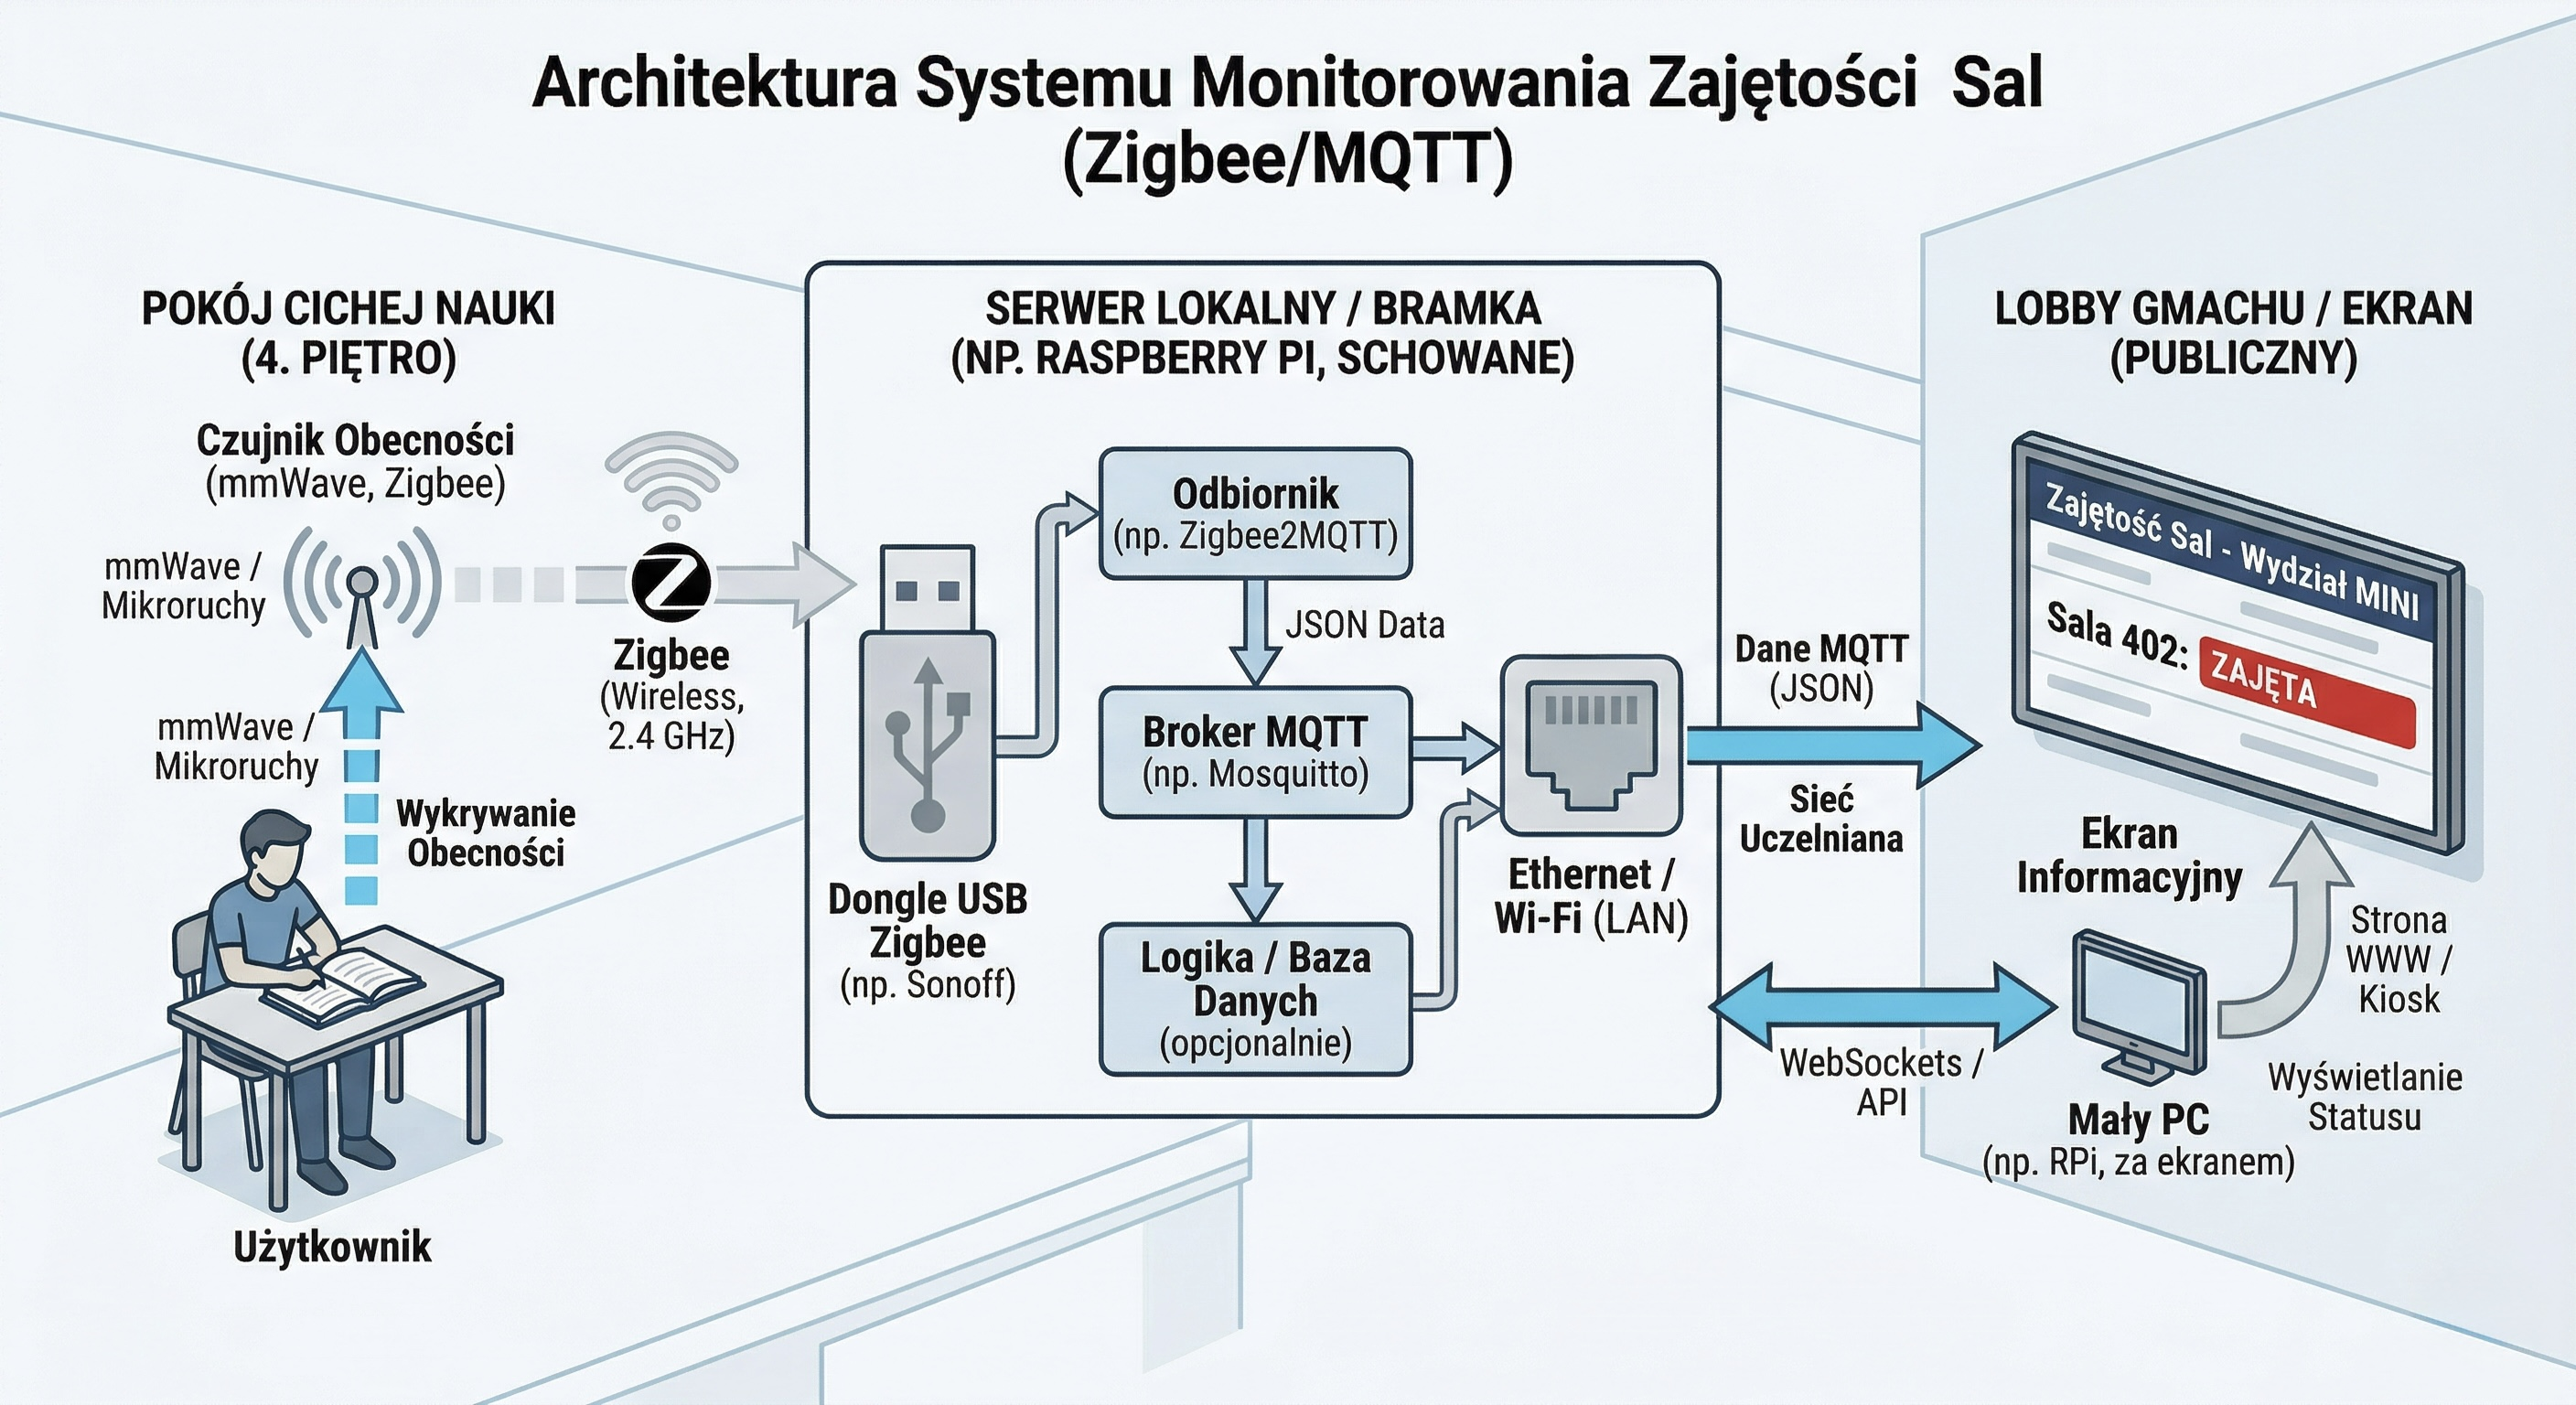
\includegraphics[width=\textwidth]{architektura.jpg}
    \caption{Architektura Systemu Monitorowania Zajętości Sal w technologii Zigbee i MQTT.}
    \label{fig:architektura}
\end{figure}

Działanie całości jest bardzo proste i można je opisać w zaledwie trzech krokach przepływu informacji:

\begin{itemize}
    \item \textbf{1. Środowisko fizyczne (Pokój Nauki - lewa strona):} Czujnik (rozpoznający ruch fizyczny z radaru) wykrywa, że student siedzi przy biurku. Ponieważ używa niezwykle energooszczędnej technologii Zigbee, wysyła wynik detekcji w powietrze drogą bezprzewodową na częstotliwości 2.4 GHz.
    \item \textbf{2. Hub Główny (Serwer Ukryty - środek):} Gdzieś dalej w budynku schowany jest malutki mikrokomputer nadzorczy (np. tanie, małe Raspberry Pi). Posiada on wetknięty do gniazda "gwizdek" USB (dongle przypominający pendrive), który świetnie radzi sobie z przechwytywaniem tych sygnałów z powietrza. Kiedy komputer je wyłapie, specjalne programy narzędziowe (np. protokół MQTT) tłumaczą surowy szum antenowy na klasyczny, ludzki tekst komputerowy typu "stan: obecność" i wgrywają to do głównej, twardej sieci ethernetowej uczelni.
    \item \textbf{3. Klient Końcowy (Z publicznym ekranem - prawa strona):} Sam wielki telewizor w holu wyposażony jest po prostu w kolejny minikomputer stykający się ze stroną WWW. Ten komputer w holu nie przeprowadza detekcji ani żadnych skomplikowanych obliczeń radarów i anten – jest stacją wyjściową. Przez internet co chwilę komunikuje się dyskretnie z Serwerem Ukrytym i na podstawie gotowego już wyniku po prostu maluje duży pasujący kafelek statusu ("Sala: Zajęta") prosto w oczy mijających go potoków studentów.
\end{itemize}

Rozbicie fizyki na te trzy elementy sprzętowe mocno upraszcza pisanie każdej linijki kodu oraz pozwala np. zresetować duży ekran w holu bez przerywania analizy liczenia wejściówek do stref nauki.

\end{document}
